

%---------------------------------------------
\newpage % NOTE: The appendix title should be on its own page.
%---------------------------------------------
\chapter{Time-Lapse Movies} \newpage
\section{Early Season} 
\href{https://youtu.be/f_LF7-_opkc}{https://youtu.be/f\_LF7-\_opkc} 
\section{Mid Season} 
\href{https://youtu.be/J5fFBARJAu0}{https://youtu.be/J5fFBARJAu0}
\section{Late Season - Isothermal Development} 
\href{https://youtu.be/hLevt5xeN9o}{https://youtu.be/hLevt5xeN9o}

\chapter{BSTA Technical Details} \newpage
\section{Parts List}
\href{https://drive.google.com/file/d/1wrSelvj6EzlNViaM0zonwLIbumqkNpm5/view?usp=sharing}{https://drive.google.com/file/d/1wrSelvj6EzlNViaM0zonwLIbumqkNpm5/ \\ view?usp=sharing}
\section{CR1000 Code}
\href{https://drive.google.com/file/d/1Z6SDvXJ5vwWH153xJffSQQ8yu_DaKKHo/view?usp=sharing}{https://drive.google.com/file/d/1Z6SDvXJ5vwWH153xJffSQQ8yu_DaKKHo/ \\ view?usp=sharing}

\section{Structure Design}
The Banner Summit Thermocouple Array is based off designs shared by Charlie Luce and Tom Black during correspondence on October 18th, 2018. We used these diagrams to design and construct the BSTA frame as seen in the below figure. Thin wires run between the two 3" channel vertical supports every 5cm and are attached to eye-bolts on each of the vertical supports. Each of these wires supports a thermocouple and is kept taught by springs on each of the eye-bolts. A 1.25m x 1.25m square of 3" channel is attached to the vertical supports and burried just below the soil to act as a foundation for the instrument. 
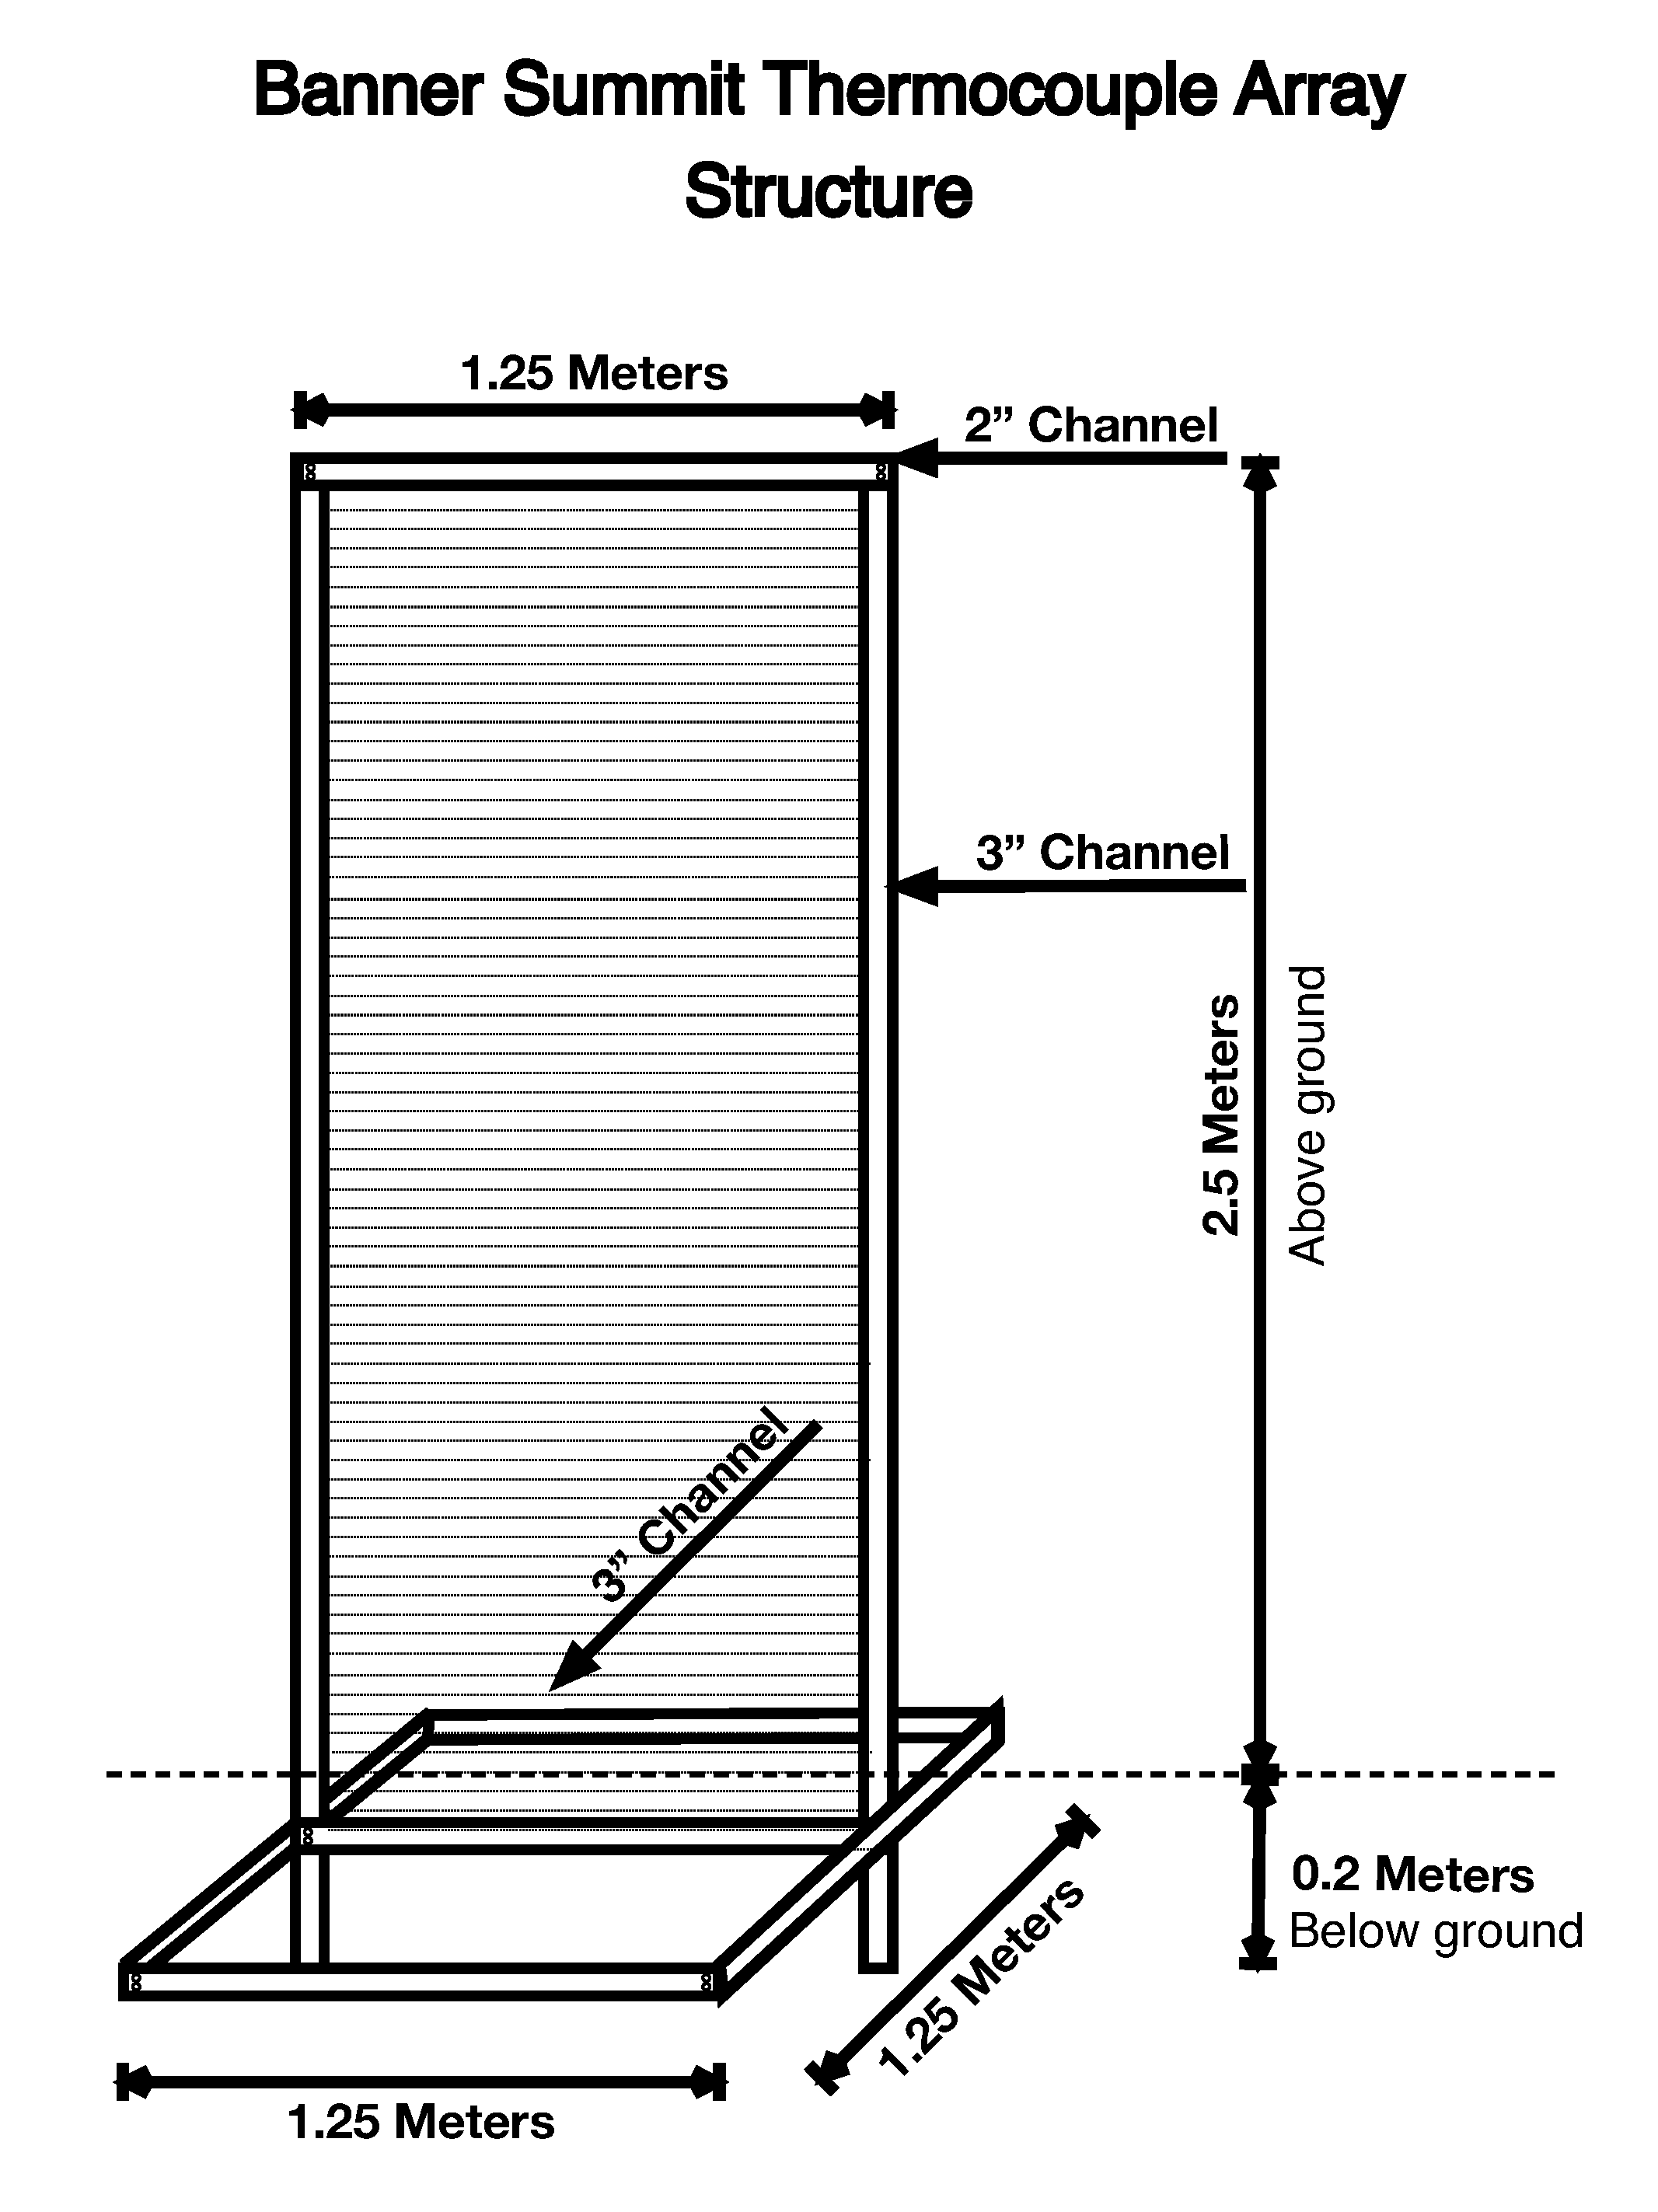
\includepdf[scale=0.8]{BSTA_Structure.pdf}

\chapter{Data \& Analysis} \newpage
\section{Water Year 2019 Data}
\href{https://drive.google.com/file/d/1S0TLlX7pi3IJApxP7INtTE2Y9EOZIk_5/view?usp=sharing}{https://drive.google.com/file/d/1S0TLlX7pi3IJApxP7INtTE2Y9EOZIk\_5/view? \\ usp=sharing}
\section{Water Year 2020 Data}
\subsection{Raw Transmitted Data}
Transmitted data from 2020 can be found via this link: \\
\href{http://denali.micro-specialties.com/cgi-bin/globalModemData.cgi?site=sn314&start=2020/2/1}{http://denali.micro-specialties.com/cgi-bin/globalModemData.cgi? \\ site=sn314&start=2020/2/1} \\ 

\subsection{2020 Data Intake (Python)}
Here is a Python script that collects transmitted data and conducts basic visualization:
\href{https://drive.google.com/file/d/1bp4srHlA0cArIyqv09bc1su8xadS9i5j/view?usp=sharing}{https://drive.google.com/file/d/1bp4srHlA0cArIyqv09bc1su8xadS9i5j/ \\ view?usp=sharing}

\section{Analysis}
Below are links to the MATLAB scripts used to conduct analysis on temperature gradients, uncertainty, and runoff timing. They are all compatable with the Water Year 2019 data found in Appendix C.1. 
\subsection{Temperature Gradient Analysis}
\href{https://drive.google.com/file/d/1q9dmvjT9bsjzyus962ExAWQKkBX-zMRJ/view?usp=sharing}{https://drive.google.com/file/d/1q9dmvjT9bsjzyus962ExAWQKkBX-zMRJ/ \\ view?usp=sharing}
\subsection{Uncertainty Analysis}
\href{https://drive.google.com/file/d/1h_b1s3D6DkYiPE2lqnu2pnMlw3HFXLCw/view?usp=sharing}{https://drive.google.com/file/d/1h_b1s3D6DkYiPE2lqnu2pnMlw3HFXLCw/ \\ view?usp=sharing}
\subsection{Isothermal Snowpack and Runoff Timing}
\href{https://drive.google.com/file/d/1dVCQnMA9SbabyH32f5AAHxmj1dchDZLI/view?usp=sharing}{https://drive.google.com/file/d/1dVCQnMA9SbabyH32f5AAHxmj1dchDZLI/ \\ view?usp=sharing}

\chapter{Stable Water Isotope Analysis} \newpage
\section{Literature Review} 
Stable water isotopes can be used to better understand snow hydrological processes (\cite{beria_larsen_ceperley_michelon_vennemann_schaefli_2017}). The effect of different snow ablation processes (sublimation, melting, and redistribution) can be seen in the isotopic evolution of a seasonal snowpack (\cite{beria_larsen_ceperley_michelon_vennemann_schaefli_2017}). Water Isotopes represent a potential independent measure of sublimation in seasonal snow cover, although the majority of work in this area has focused on hydrograph separation (\cite{gustafson2010estimating}). Sommerfel (1987) and Gustafson (2010) found that isotope fractionation, driven by high vapor pressure deficits, could be a sensitive tool for determining relative mass change in a column of snow. However, other studies have failed to prove the ability of water isotopes to gauge water loss due to sublimation (\cite{friedman1991isotopic}). 

Spatial precipitation patterns, preferential snow deposition, and wind redistribution lead to heterogeneous snow accumulation patterns (\cite{beria_larsen_ceperley_michelon_vennemann_schaefli_2017}). Complex interactions among snow ablation, topography, and vegetation lead to more spatial heterogeneity of snow packs (\cite{beria_larsen_ceperley_michelon_vennemann_schaefli_2017}). The spatial variability associated with snowpack stable water isotopes poses a significant challenge when using it as an independent measure of sublimation in seasonal snow cover. 

\section{Methods}
Snow was sampled within 20 meters of the Banner Summit SNOTEL site for analysis of stable water isotopes. The snow pit locations are randomly selected on a flat surface with no apparent aspect. The sampled area is lightly forested, but care is taken in order to prevent contamination from secondary snow input such as fallen, intercepted snow or wind drifts. In order to capture the full isotopic content of a snowpack, samples were collected from the whole snow profile with a 3cm vertical resolution. To assess spatial variability of stable water isotopes, duplicate samples were collected from one pit with about 0.5 m horizontal spacing (figure \ref{fig:Pit_18Dec19}). To assess systematic bias in the sampling method, samples were collected in triplicates directly adjacent to each other (figure \ref{fig:Pit_17Mar19}). Detailed notes are taken on snowpack characteristics during each sampling event.

Snow samples are transported back to Boise State University where they are stored at -20°C. A fourth generation (purchased 2011) Los Gatos Research (LGR) Liquid Water Isotope Analyzer (LWIA) is used to measure \textsuperscript{2}H/\textsuperscript{1}H and \textsuperscript{18}O/\textsuperscript{16}O for all snow samples. Results are reported in units of per mil (\textperthousand), relative to Vienna Standard Mean Ocean Water (VSMOW). Raw LWIA values are processed using the Los Gatos Research post-processing software.

 \begin{figure}[H]
    \centering
    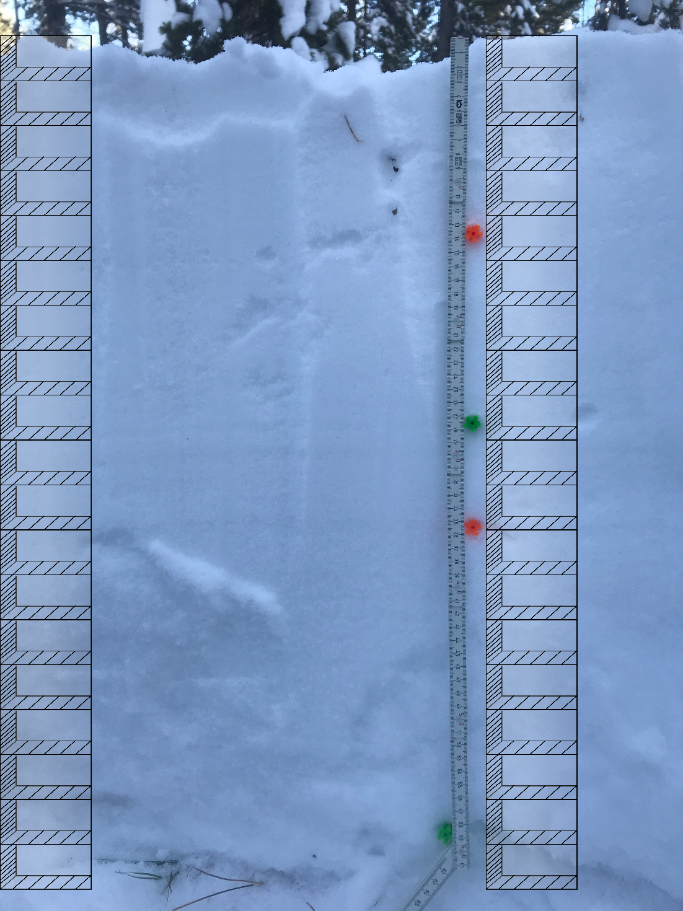
\includegraphics[width=0.4\linewidth]{figures/Pit_18Dec19.png}
    \caption{Picture of the sampling pit used on December 18, 2018 illustrating where duplicates were sampled with about 0.5m spacing as represented by the shaded boxes with black lines. The red and green dots are observed ice layers, and storm layer surfaces.}
    \label{fig:Pit_18Dec19}
 \end{figure}
 
 \begin{figure}[H]
    \centering
    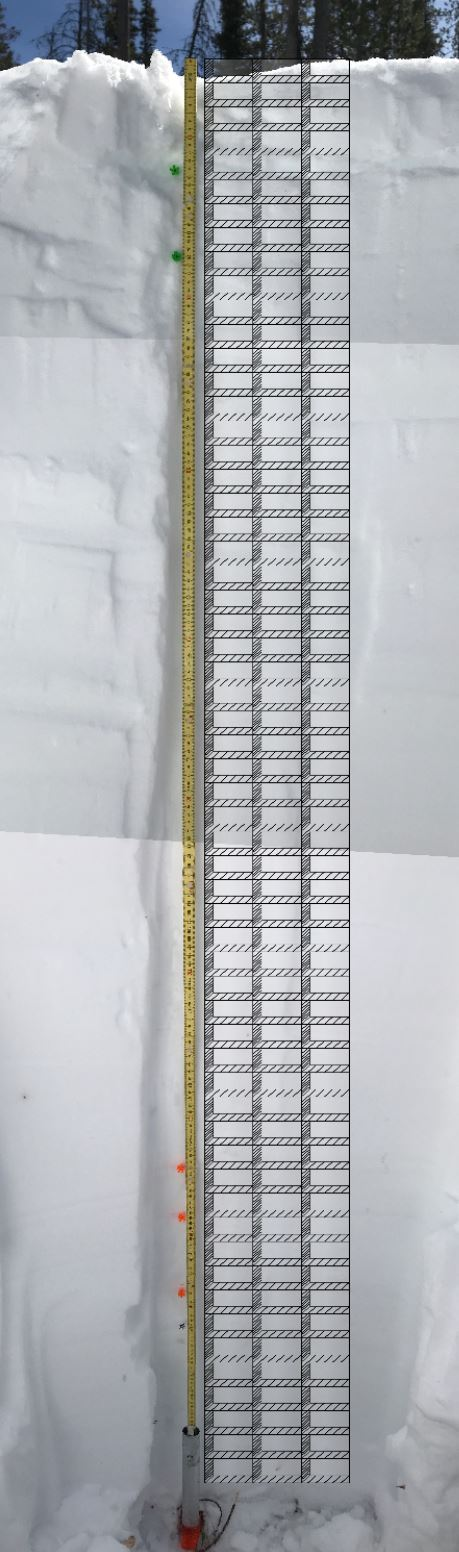
\includegraphics[width=0.3\linewidth]{figures/Pit_17Mar19.jpg}
    \caption{Picture of the sampling pit used on March 17th, 2019 showing where triplicates were collected.}
    \label{fig:Pit_17Mar19}
 \end{figure}
 
\section{Results}
Early in the season, duplicate snow samples were taken from a single pit, but with ~0.5m horizontal spacing (\ref{fig:Pit_18Dec19}). This resulted in significant differences (up to 50\%) in stable isotopes near the top of the snowpack (\ref{fig:Dec18_Isotopes}). The variation between duplicates was much lower in the bottom of the snowpack. Similar trends are present in each duplicate, just displaced with respect to depth. Later in the season, Mar. 17th, triplicate samples were taken directly adjacent to each other (\ref{fig:Pit_17Mar19}) and the results suggest very little variation between triplicates with a maximum difference of 13\% (\ref{fig:Mar17_Isotopes}). 

\begin{figure}[H]
    \centering
    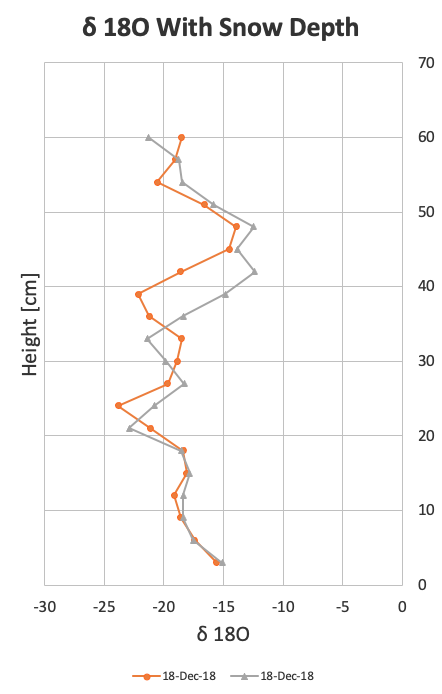
\includegraphics[width=0.7\linewidth]{figures/Isotopes/Dec18_Isotopes.png}
    \caption{Stable water isotope composition for samples taken on December 18, 2018. There is strong agreement in the lowest 10cm, but the profiles diverge moving up through the snowpack. The largest difference between profiles is right around 40cm.}
    \label{fig:Dec18_Isotopes}
\end{figure}

\begin{figure}[H]
    \centering
    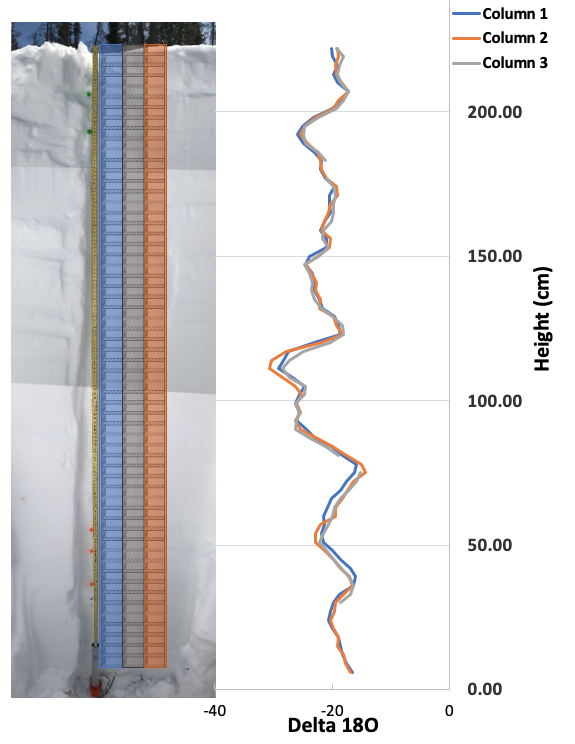
\includegraphics[width=0.7\linewidth]{figures/Isotopes/Mar17_Isotopes.png}
    \caption{Stable water isotope composition for samples taken on March 17, 2019.}
    \label{fig:Mar17_Isotopes}
\end{figure}

\section{Discussion}
 Samples for stable isotope analysis were collected in a lightly forested area with varying amounts of underbrush and fallen trees. This uneven ground creates an inconsistent datum between sampling events and introduces an unexpected amount of spatial variability. In addition to this, the presence of vegitation also affects snow processes via emission of longwave radiation, screening of solar radiation, etc (\cite{beria_larsen_ceperley_michelon_vennemann_schaefli_2017}. Moving forward, sampling for stable water isotopes in snow should be conducted in open areas with an even ground surface that is free of large brush, or fallen debris. If a study is conducted in a forested/lightly forested area, there should be a preseason effort to clear the sampling locations of anything that creates an uneven ground surface. 

Although this dataset does not provide a basis for conclusions that differ from previous studies, there are important trends to note. Figure \ref{fig:WY2019_Isotopes} shows samples taken from three different days accross the season. The $\delta$\textsuperscript{18}O values are more consistent in the lowest portion of the snowpack and diverge upwards. 

\begin{figure}
    \centering
    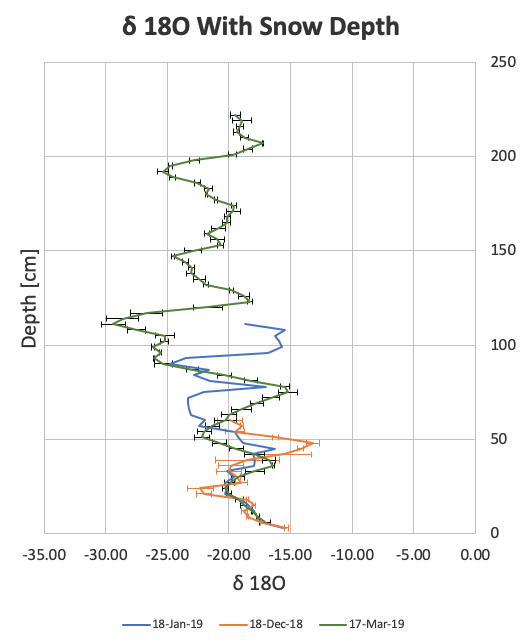
\includegraphics[width=0.8\linewidth]{figures/Isotopes/Season_Isotopes.png}
    \caption{Oxygen isotopes sampled throughout the 2019 winter season.}
    \label{fig:WY2019_Isotopes}
 \end{figure}

\section{Conclusions}
Any time there is a phase change with subsequent migration of water molecules, the stable water isotope concentrations of the remaining snow is altered. Measuring this change in stable isotope concentrations over time could improve our current understanding of internal snowpack processes. Future work should focus on reducing the error associated with sampling snow over a sizeable temporal domain. Improving our identification of specific storm layers will increase our ability to correlate between sampling events and will improve our ability to interpret this data. Additionally, establishing a snow sampling regime with a consistent datum, or ground surface, will reduce the error.   